%%%%%%%%%%%%%%%%%%%%%%%%%%%%%%%%%%%%%%%%%
% Beamer Presentation
% LaTeX Template
% Version 1.0 (10/11/12)
%
% This template has been downloaded from:
% http://www.LaTeXTemplates.com
%
% License:
% CC BY-NC-SA 3.0 (http://creativecommons.org/licenses/by-nc-sa/3.0/)
%
%%%%%%%%%%%%%%%%%%%%%%%%%%%%%%%%%%%%%%%%%

%----------------------------------------------------------------------------------------
%	PACKAGES AND THEMES
%----------------------------------------------------------------------------------------

\documentclass{beamer}

\mode<presentation> {

% The Beamer class comes with a number of default slide themes
% which change the colors and layouts of slides. Below this is a list
% of all the themes, uncomment each in turn to see what they look like.

%\usetheme{default}
%\usetheme{AnnArbor}
%\usetheme{Antibes}
%\usetheme{Bergen}
%\usetheme{Berkeley}
%\usetheme{Berlin}
%\usetheme{Boadilla}
%\usetheme{CambridgeUS}
%\usetheme{Copenhagen}
%\usetheme{Darmstadt}
%\usetheme{Dresden}
%\usetheme{Frankfurt}
%\usetheme{Goettingen}
%\usetheme{Hannover}
%\usetheme{Ilmenau}
%\usetheme{JuanLesPins}
%\usetheme{Luebeck}
\usetheme{Madrid}
%\usetheme{Malmoe}
%\usetheme{Marburg}
%\usetheme{Montpellier}
%\usetheme{PaloAlto}
%\usetheme{Pittsburgh}
%\usetheme{Rochester}
%\usetheme{Singapore}
%\usetheme{Szeged}
%\usetheme{Warsaw}

% As well as themes, the Beamer class has a number of color themes
% for any slide theme. Uncomment each of these in turn to see how it
% changes the colors of your current slide theme.

%\usecolortheme{albatross}
%\usecolortheme{beaver}
%\usecolortheme{beetle}
%\usecolortheme{crane}
%\usecolortheme{dolphin}
%\usecolortheme{dove}
%\usecolortheme{fly}
%\usecolortheme{lily}
%\usecolortheme{orchid}
%\usecolortheme{rose}
%\usecolortheme{seagull}
%\usecolortheme{seahorse}
%\usecolortheme{whale}
%\usecolortheme{wolverine}

%\setbeamertemplate{footline} % To remove the footer line in all slides uncomment this line
%\setbeamertemplate{footline}[page number] % To replace the footer line in all slides with a simple slide count uncomment this line

%\setbeamertemplate{navigation symbols}{} % To remove the navigation symbols from the bottom of all slides uncomment this line
}

\usepackage{graphicx} % Allows including images
\usepackage{booktabs} % Allows the use of \toprule, \midrule and \bottomrule in tables

\usepackage[utf8]{inputenc} % Tällä toimii utf-8
\usepackage[T1]{fontenc}      % Ja tämä liittyy edelliseen
\usepackage[english]{babel} %Suomenkielinen tavutus
%\usepackage{tytiivis} %Tiivistelmäsivun laatimiseksi
%\usepackage[dvips]{graphicx}%Saadaan kuvat toimimaan %I commented
\usepackage{lastpage}
\usepackage{amsmath}
\usepackage{amssymb}
\usepackage{gensymb}

%###
\usepackage{epsfig}
\usepackage{times}
\usepackage{enumerate}
\usepackage{float}
\usepackage{epstopdf}
\usepackage{amsfonts}

\addto\captionsfinnish{%
  \renewcommand{\refname}%
    {References}%   
}


\addto\captionsfinnish{%
  \renewcommand{\contentsname}%
    {Contents}%
}

\addto\captionsfinnish{%
  \renewcommand{\figurename}%
    {Figure}%
}

\addto\captionsfinnish{%
  \renewcommand{\tablename}%
    {Table}%
}

\def\rg{r_{\rm S}} % Schwarzschild radius

\def\be{\begin{equation}}
\def\ee{\end{equation}}
\def\bc{\begin{center}}
\def\ec{\end{center}}
\def\beq{\begin{eqnarray}}
\def\eeq{\end{eqnarray}}

\def\msun{{\rm M_{\odot}}}
\def\d{{\rm d}}
\def\Ledd{L_{\rm Edd}}
\def\xte{{\it RXTE}}
\def\Ginga{{\it Ginga}}
%\def\deg{^{\circ}}
\def\rinf{r_{\rm spot, \infty}}
\def\Tinf{T_{\infty}}
\def\Te{T_{\rm e}}
\def\phip{\phi_{\rm p}}
\def\phis{\phi_{\rm s}}
\def\alphap{\alpha_{\rm p}}
\def\alphas{\alpha_{\rm s}}
%\def\muv{\mu_{\rm v}}

\def\rg{r_{\rm S}} % Schwarzschild radius
\def\betaeq{\beta_{\rm eq}}
%\def\Dop{{\cal{D}}}
\def\Dop{\delta}
\def\taut{\tau_{\rm es}}
\def\source{SAX J1808.4$-$3658}
\def\sourceb{SAX J1748.9$-$2021}
\def\mumin{\mu_{\rm min}}
\def\mumax{\mu_{\rm max}}
\def\phiobs{\phi_{\rm obs}}
\def\ani{h}
\def\thetas{\theta_{s}}
\def\tstep{\mathsf{t}}
%###






%----------------------------------------------------------------------------------------
%	TITLE PAGE
%----------------------------------------------------------------------------------------

%\title[Short title]{Mass and radius constraints for neutron stars from pulse shape modeling } % The short title appears at the bottom of every slide, the full title is only on the title page
\title{Mass and radius constraints for neutron stars from pulse shape modeling }


\author{Tuomo Salmi} % Your name
\institute[UTU] % Your institution as it will appear on the bottom of every slide, may be shorthand to save space
{
University of Turku \\ % Your institution for the title page
\medskip
\textit{thjsal@utu.fi} % Your email address
}
%\date{\today} % Date, can be changed to a custom date

\begin{document}

\begin{frame}
\titlepage % Print the title page as the first slide
\end{frame}

%\begin{frame}
%\frametitle{Overview} % Table of contents slide, comment this block out to remove it
%\tableofcontents % Throughout your presentation, if you choose to use \section{} and \subsection{} commands, these will automatically be printed on this slide as an overview of your presentation
%\end{frame}

%----------------------------------------------------------------------------------------
%	PRESENTATION SLIDES
%----------------------------------------------------------------------------------------

%------------------------------------------------
%\section{First Section} % Sections can be created in order to organize your presentation into discrete blocks, all sections and subsections are automatically printed in the table of contents as an overview of the talk
%------------------------------------------------

%\subsection{Subsection Example} % A subsection can be created just before a set of slides with a common theme to further break down your presentation into chunks

\begin{frame}
\frametitle{Aim}
\begin{itemize}
\item Determination of masses and radii for rapidly rotating neutron stars 
\item Constrain the number of possible equations of state
\item The properties of matter at extremely high densities
\item Study the effects of polarization measurements on mass and radius constraints
\end{itemize}
\end{frame}

\begin{frame}
\frametitle{Contents}
%\begin{minipage}{0.5\textwidth}
\begin{itemize}
\item Introduction
\begin{itemize}
\item Neutron stars
\item Accreting millisecond pulsars
\end{itemize}
\item Methods
\begin{itemize}
\item Modeling the pulse profiles of accreting millisecond pulsars
\item Bayesian inference and Monte Carlo sampling methods
\item Test our tools and methods with synthetic data
\end{itemize}
\item Results
\begin{itemize}
\item Polarization measurements may be used the get
significantly tighter constraints for masses and radii. 
\end{itemize}
\end{itemize}
%\end{minipage}%
%\begin{minipage}{.5\textwidth}
%\begin{figure}
%\includegraphics[width=0.7\linewidth]{neutron-star-magnetic-field.jpg}
%\end{figure}
%\end{minipage}
\end{frame}




\begin{frame}
\frametitle{Neutron stars}
\begin{itemize}
\item Most dense objects that can be directly observed
\item Typical mass $M = 1.5 M_{\odot}$ and typical radius $R =  12$ km
\item Supernuclear densities (5 to 10 times the nuclear equilibrium density $n_{0} \approx 0.16 ~\mathrm{fm}^{-3}$ of neutrons and protons)
\item Are created after the gravitational collapse of a core of a
massive star ($> 8 M_{\odot}$) at the end of its life.
\end{itemize}
\end{frame}

%------------------------------------------------

\begin{frame}
\frametitle{Neutron stars}
\begin{minipage}{0.5\textwidth}
\begin{itemize}
\item Composition of the innermost core is unknown.
\item Equation of state (EOS) gives the relation between the pressure and density (or mass and radius).
\item The EOS of a neutron star is unknown.
\end{itemize}
\end{minipage}%
\begin{minipage}{.5\textwidth}
\begin{figure}
%\includegraphics[width=0.7\linewidth]{neutron-star-magnetic-field.jpg}
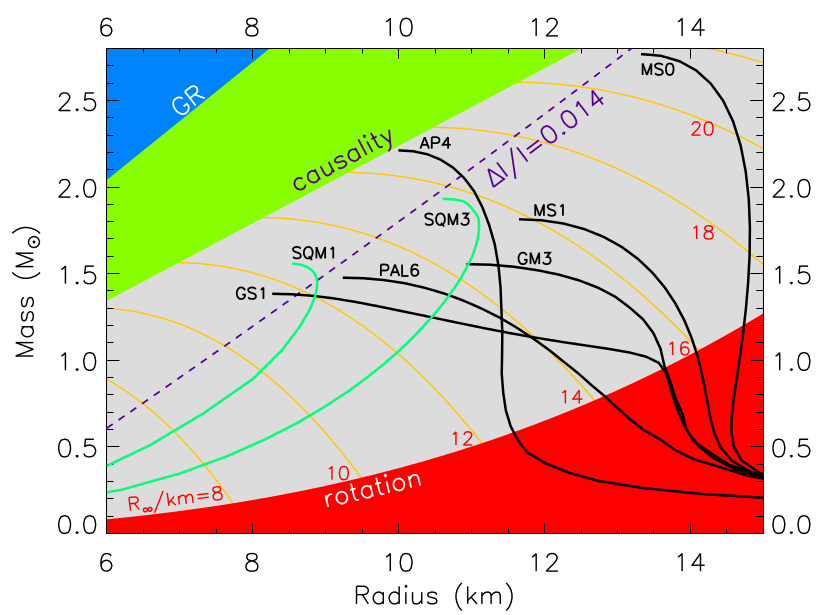
\includegraphics[width=1.1\linewidth]{eos_mr.png}
\caption{Figure 2 from Lattimer and Prakash (2004).}
\end{figure}
\end{minipage}
\end{frame}


%------------------------------------------------


%------------------------------------------------

\begin{frame}
\frametitle{Neutron stars}
\begin{minipage}{0.5\textwidth}
\begin{itemize}
\item Observed masses and radii constrain the number of possible EOSs.
\item Upper limits for compactness
\begin{itemize}
\item The general relativity (Schwarzschild condition)
\item Causality condition
\end{itemize}
\item Lower limit for compactness
\begin{itemize}
\item Fastest observed rotational frequency 
\end{itemize}
\end{itemize}
\end{minipage}%
\begin{minipage}{.5\textwidth}
\begin{figure}
%\includegraphics[width=0.7\linewidth]{neutron-star-magnetic-field.jpg}
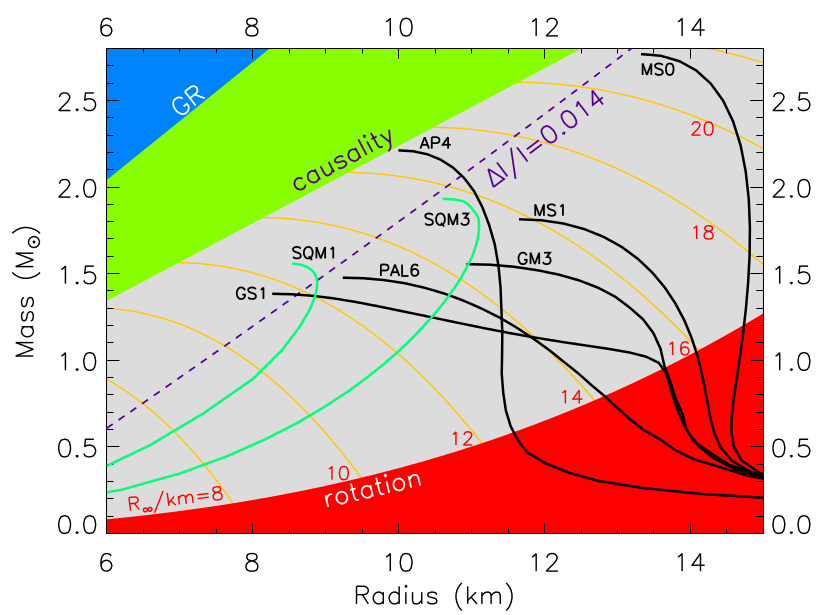
\includegraphics[width=1.1\linewidth]{eos_mr.png}
\caption{Figure 2 from Lattimer and Prakash (2004).}
\end{figure}
\end{minipage}
\end{frame}


%------------------------------------------------



%\begin{frame}
%\frametitle{Bullet Points}
%\begin{itemize}
%\item Lorem ipsum dolor sit amet, consectetur adipiscing elit

%\end{itemize}
%\end{frame}

%------------------------------------------------

%\begin{frame}
%\frametitle{Blocks of Highlighted Text}
%\begin{block}{Block 1}
%Lorem ipsum dolor sit amet, consectetur adipiscing elit. Integer lectus nisl, ultricies in feugiat %rutrum, porttitor sit amet augue. Aliquam ut tortor mauris. Sed volutpat ante purus, quis accumsan %dolor.
%\end{block}

%\begin{block}{Block 2}
%Pellentesque sed tellus purus. Class aptent taciti sociosqu ad litora torquent per conubia nostra, %per inceptos himenaeos. Vestibulum quis magna at risus dictum tempor eu vitae velit.
%\end{block}

%\begin{block}{Block 3}
%Suspendisse tincidunt sagittis gravida. Curabitur condimentum, enim sed venenatis rutrum, ipsum %neque consectetur orci, sed blandit justo nisi ac lacus.
%\end{block}
%\end{frame}

%------------------------------------------------

\begin{frame}
\frametitle{Neutron stars}
\begin{columns}[c] % The "c" option specifies centered vertical alignment while the "t" option is used for top vertical alignment

\column{.45\textwidth} % Left column and width
%\textbf{Heading}
%\begin{enumerate}
%\item Statement
%\item Explanation
%\item Example
%\end{enumerate}
\begin{itemize}
\item The highest observed mass rules out many EOSs.
\item We aim to find out independent knowledge of both mass and radius.
\end{itemize}


\column{.5\textwidth} % Right column and width
\begin{figure}
%\includegraphics[width=0.7\linewidth]{neutron-star-magnetic-field.jpg}
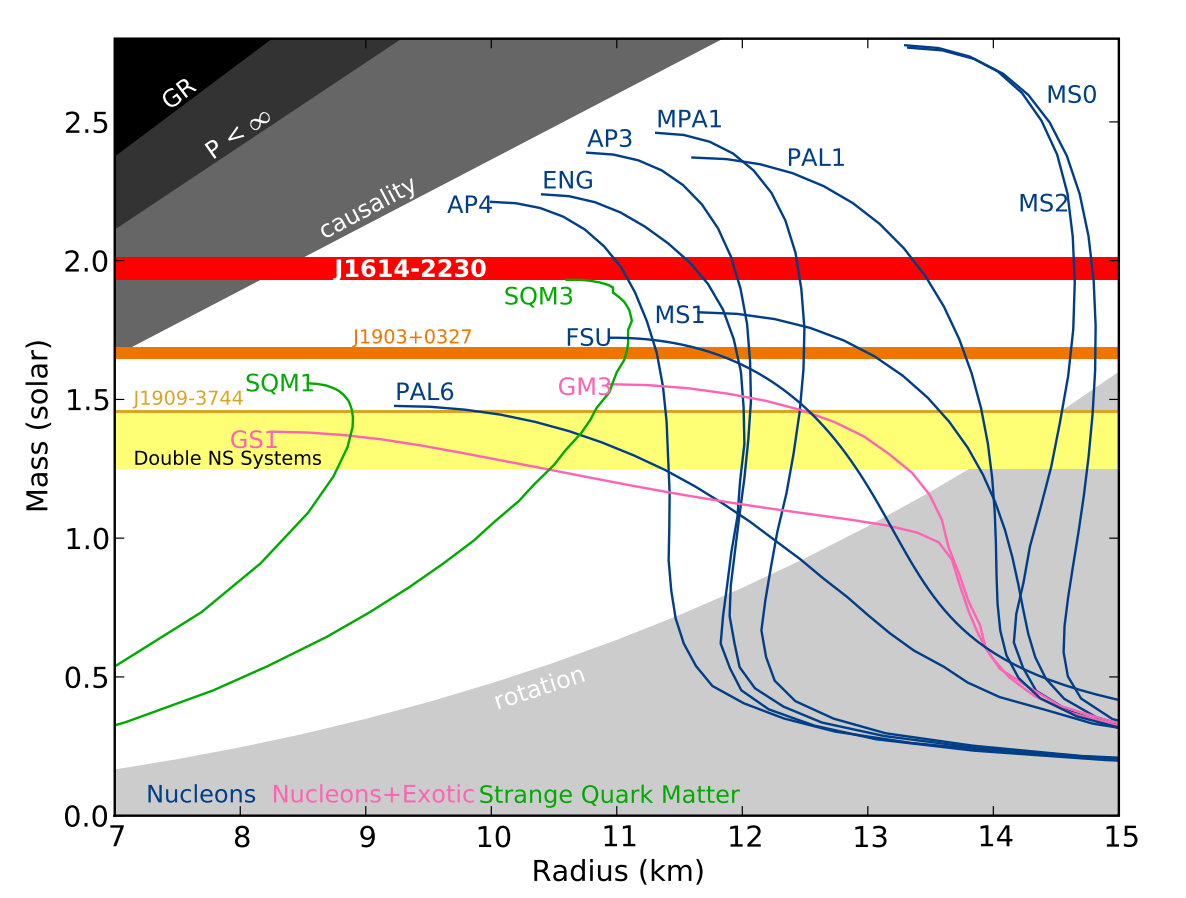
\includegraphics[width=1.1\linewidth]{eos_mr2.png}
\caption{Figure from Demorest et al. (2010).}
\end{figure}

\end{columns}
\end{frame}







\begin{frame}
\frametitle{Accreting millisecond X-ray pulsars (AMXP)}
\begin{columns}[c] % The "c" option specifies centered vertical alignment while the "t" option is used for top vertical alignment

\column{.45\textwidth} % Left column and width
\begin{itemize}
\item A subgroup of low mass X-ray binaries (LMXB)
\item Gas from the accretion disk (stripped from the companion) is channeled onto the magnetic poles of a millisecond pulsar.
\item A pair of "hot spots"
\end{itemize}


\column{.5\textwidth} % Right column and width
\begin{figure}
%\includegraphics[width=0.7\linewidth]{neutron-star-magnetic-field.jpg}
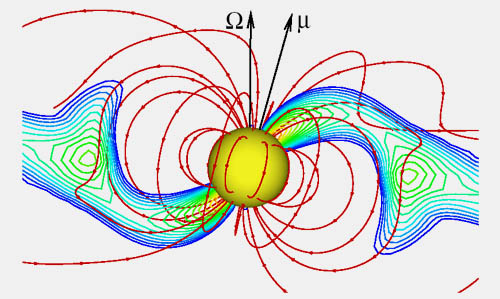
\includegraphics[width=1.1\linewidth]{schematic.jpg}
\caption{Figure 4 from Romanova et. al (2004).}
\end{figure}

\end{columns}
\end{frame}

\begin{frame}
\frametitle{Accreting millisecond X-ray pulsars (AMXP)}
\begin{columns}[c] % The "c" option specifies centered vertical alignment while the "t" option is used for top vertical alignment

\column{.45\textwidth} % Left column and width
\begin{itemize}
%\item Roche lobe overflow
\item Recycling scenario
\begin{itemize}
\item The evolutionary progenitors of recycled radio millisecond pulsars%From $B \sim 10^{12}$ G to $B \sim 10^{8}$ G
\end{itemize}

\end{itemize}


\column{.5\textwidth} % Right column and width
\begin{figure}
%\includegraphics[width=0.7\linewidth]{neutron-star-magnetic-field.jpg}
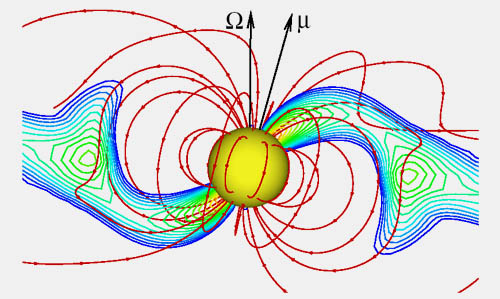
\includegraphics[width=1.1\linewidth]{schematic.jpg}
\caption{Figure 4 from Romanova et. al (2004).}
\end{figure}

\end{columns}
\end{frame}

%------------------------------------------------



\begin{frame}
\frametitle{Accreting millisecond X-ray pulsars (AMXP)}
\begin{columns}[c] % The "c" option specifies centered vertical alignment while the "t" option is used for top vertical alignment

\column{.45\textwidth} % Left column and width
\begin{itemize}
\item Some of AMXPs show outbursts
\item SAX J1808.4$-$3658: Nearly coherent oscillations detected during outbursts
\item Similar outburst evolution: SAX J1748.9$-$2021 (in the Figure)

\end{itemize}


\column{.5\textwidth} % Right column and width
\begin{figure}
%\includegraphics[width=0.7\linewidth]{neutron-star-magnetic-field.jpg}
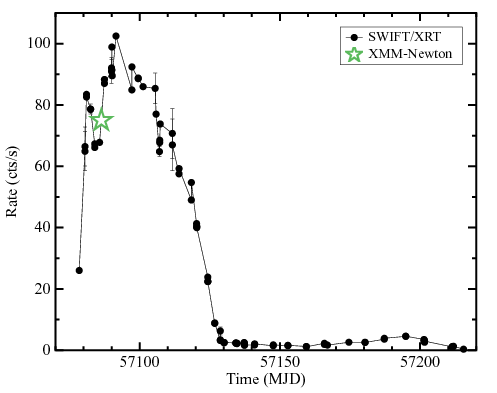
\includegraphics[width=1.1\linewidth]{outburst.png}
\caption{Figure 1 from Sanna et al. (2016).}
\end{figure}

\end{columns}
\end{frame}


%--------------------------------------------

\begin{frame}
\frametitle{SAX J1808.4$-$3658}

\begin{figure}
%\includegraphics[width=0.7\linewidth]{neutron-star-magnetic-field.jpg}
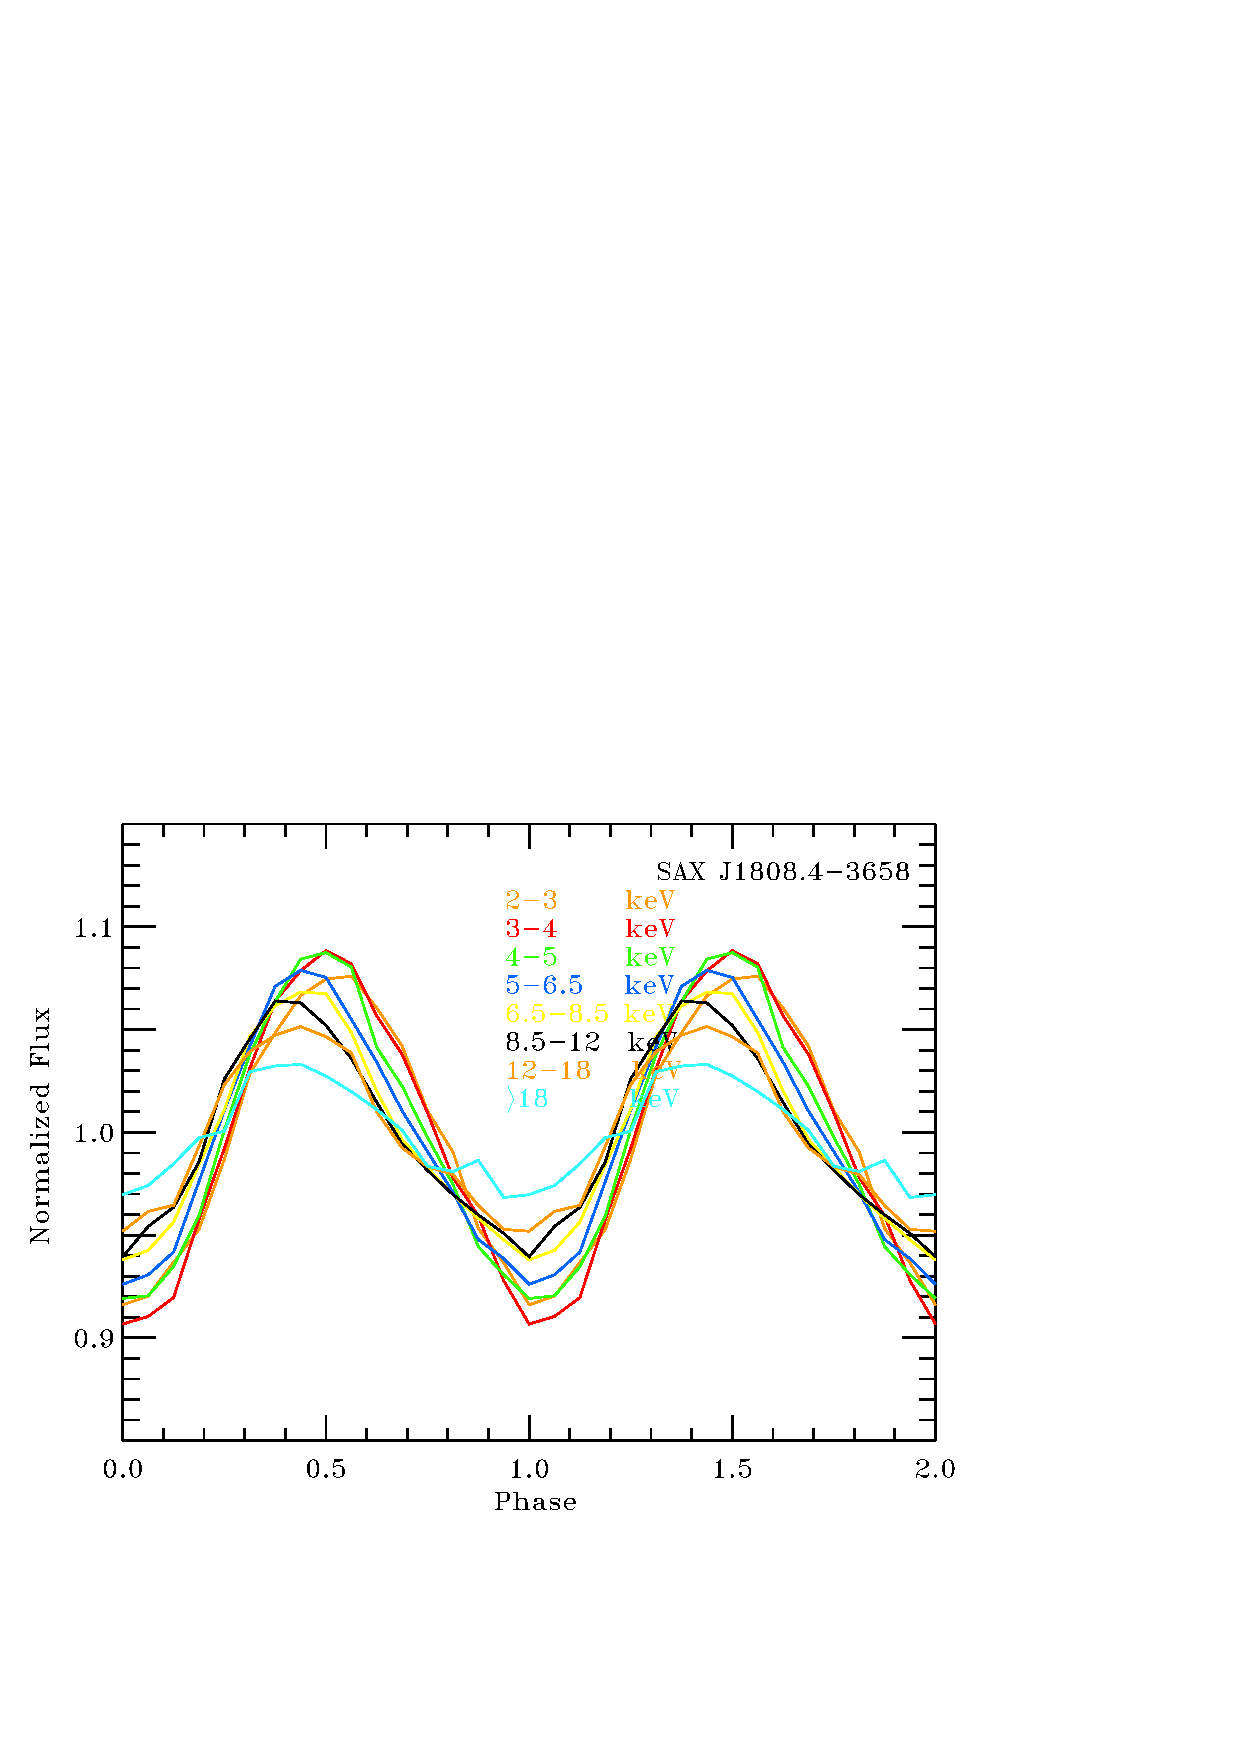
\includegraphics[width=0.8\linewidth]{data_sax1808.pdf}
%\caption{Figure 2 from Lattimer and Prakash (2004)}
\end{figure}

\end{frame}

%-----------------------------------------------------



\begin{frame}
\frametitle{Methods}
\begin{itemize}
\item Pulse shape modeling
\item Bayesian analysis
\item Monte Carlo sampling methods
\end{itemize}
\end{frame}

%--------------------------------------------



%--------------------------------------------

\begin{frame}
\frametitle{Pulse profile modeling}
\begin{columns}[t] % The "c" option specifies centered vertical alignment while the "t" option is used for top vertical alignment
\column{.45\textwidth} 
\begin{itemize}

\item Schwarzschild + Doppler approximation (S+D)
\item Oblate shape of the star taken into account
\item Mass and radius affecting the light bending
\item Time delays different from different locations 

\end{itemize}
\column{.5\textwidth} 
\begin{figure}
%\includegraphics[width=0.7\linewidth]{neutron-star-magnetic-field.jpg}
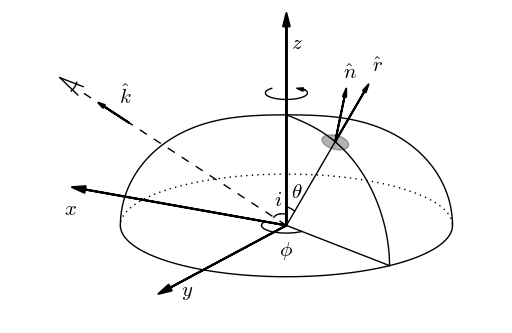
\includegraphics[width=1.1\linewidth]{fig2.png}
%\caption{Figure 2 from Lattimer and Prakash (2004)}
\end{figure}
\end{columns}
\end{frame}

%-----------------------------------------------------

%--------------------------------------------

\begin{frame}
\frametitle{Pulse profile modeling}
 
\begin{itemize}

\item Observed spectral flux from an infinitesimal spot:

\be \label{eq:fluxspot2}
\d F_{E}=(1-u)^{1/2} \Dop^{4} I'_{E'}(\sigma') \cos\sigma
\frac{\d \cos\alpha}{\d\cos\psi}
 \frac{\d S'}{D^2} 
\ee

\item $D$ = distance, $\psi$ = bending angle, $\Dop$ = Doppler factor, $(1-u)^{1/2}$ = inverse of gravitational redshift, $\sigma$  = emission angle relative to the spot normal, and $\alpha$  = emission angle relative to the radius vector.
\item Integration over the spot surface
\end{itemize}

\end{frame}

%-----------------------------------------------------



%--------------------------------------------

\begin{frame}
\frametitle{Pulse profile modeling}
\begin{columns}[t] % The "c" option specifies centered vertical alignment while the "t" option is used for top vertical alignment
\column{.45\textwidth} 
\begin{itemize}

\item Energy spectrum (energy dependency of $I'_{E'}$)
\item Blackbody + Power-law according to observations
\item Heated hot spot + Comptonization from an accretion shock
\item In this thesis two-component power-law 
\item $I'_{E'}(\sigma') \propto \sigma'$ either isotropic or "Hopf" profile

\end{itemize}
\column{.5\textwidth} 
\begin{figure}
%\includegraphics[width=0.7\linewidth]{neutron-star-magnetic-field.jpg}
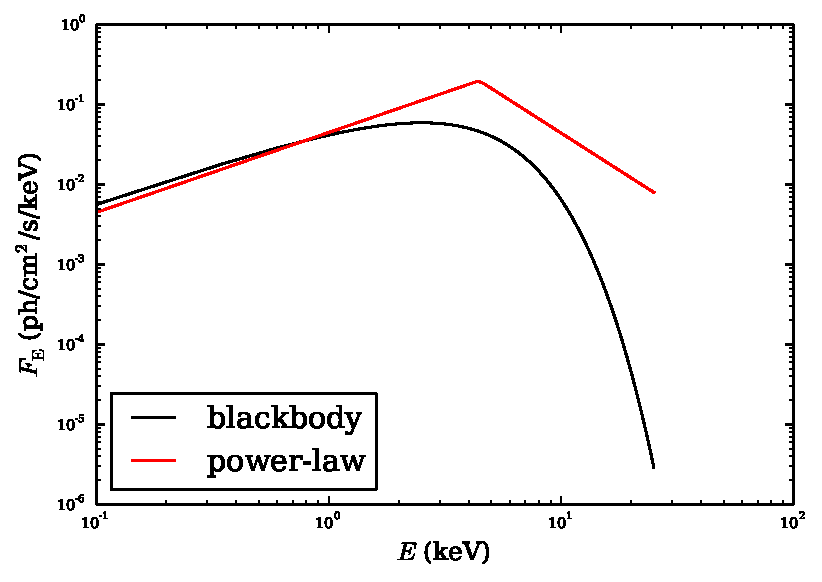
\includegraphics[width=1.1\linewidth]{spectrum_numflux0.pdf}
\end{figure}
\end{columns}
\end{frame}

%-----------------------------------------------------






%--------------------------------------------

\begin{frame}
\frametitle{SAX J1808.4$-$3658}

\begin{figure}
%\includegraphics[width=0.7\linewidth]{neutron-star-magnetic-field.jpg}
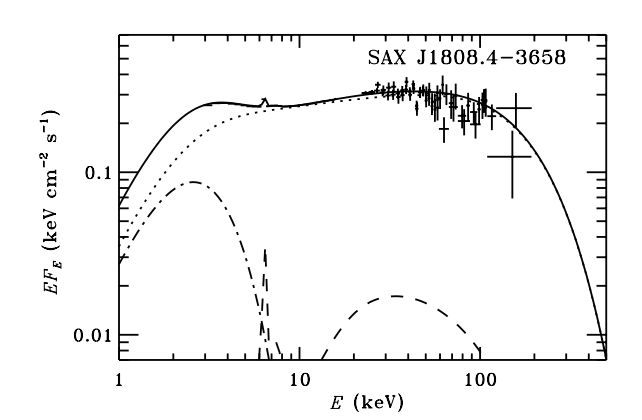
\includegraphics[width=0.8\linewidth]{spectrum_sax.png}
\caption{Figure 3 from Poutanen and Gierlinski (2003).}
\end{figure}

\end{frame}

%-----------------------------------------------------





\iffalse
%--------------------------------------------

\begin{frame}
\frametitle{Example of pulse profile comparison}

\begin{figure}
%\includegraphics[width=0.7\linewidth]{neutron-star-magnetic-field.jpg}
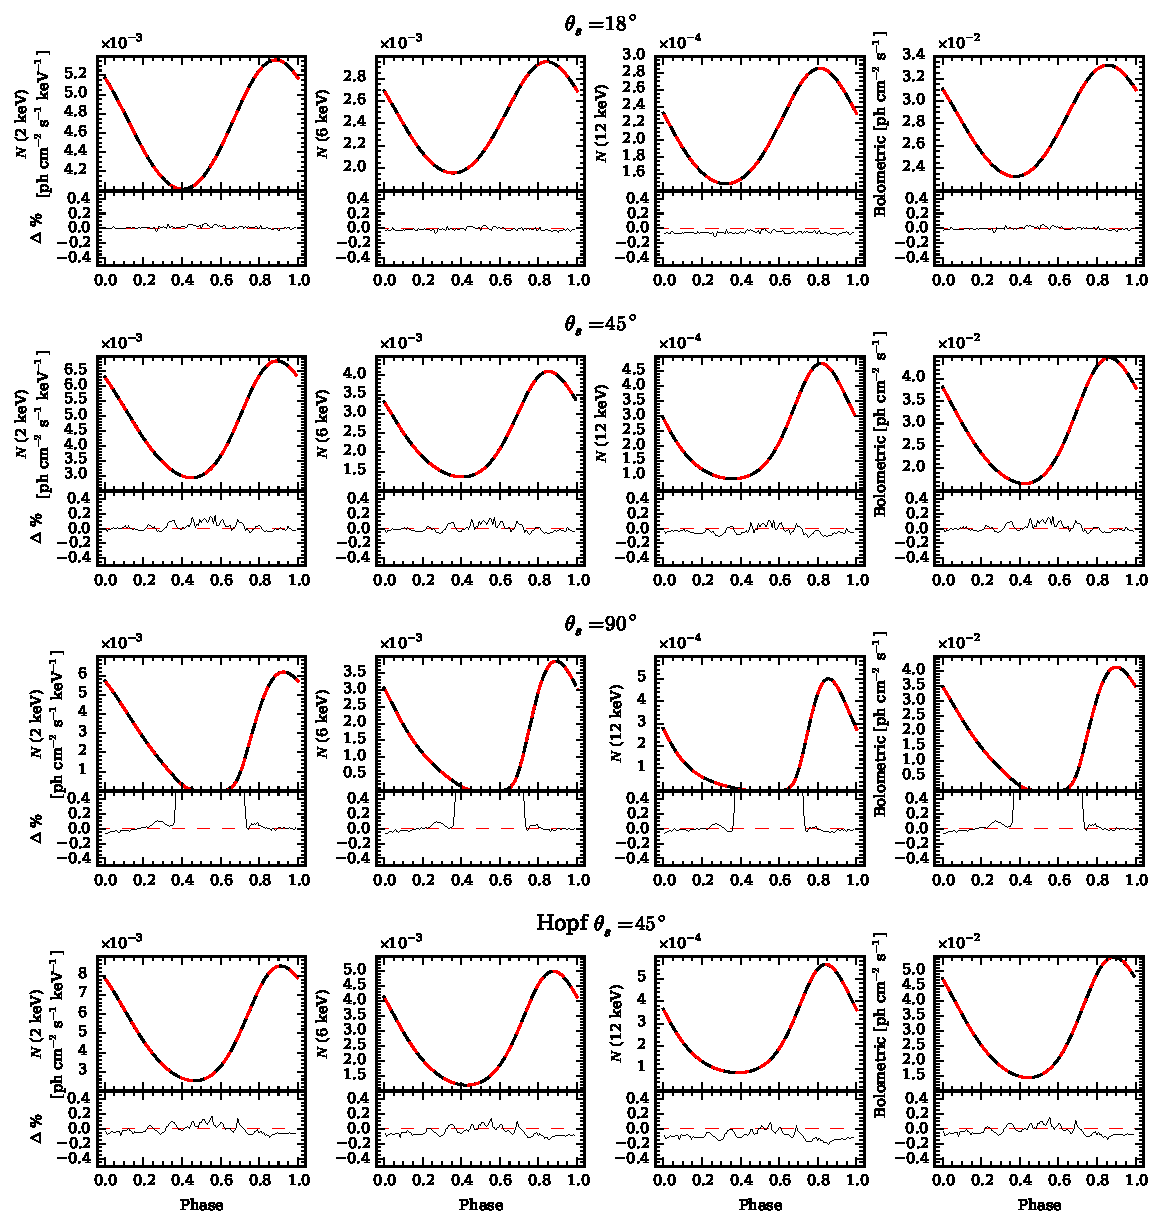
\includegraphics[width=0.5\linewidth]{jpulsec3.pdf}
\caption{The light curve comparisons with an oblate star ($R_{\mathrm{eq}} = 12$ km, $M = 1.4$ $\msun$, $\nu = 700$ Hz, $i = 45 \degree$, $\rho = 10 \degree$, and $T_{\mathrm{eff}} = 2$ keV). Figure from Nättilä and Pihajoki 2016 (in preparation).}
\end{figure}

\end{frame}

%-----------------------------------------------------
\fi




\begin{frame}
\frametitle{Bayesian inference}

\be \label{eq:bayes}
p(\textbf{y}|\mathcal{D}) \propto p(\mathcal{D}|\textbf{y})p(\textbf{y})
\ee
\begin{itemize}
\item $\mathcal{D}$ = Data
\item $\textbf{y}$ = Parameters of the pulse profile model
\item $p(\textbf{y})$ = Prior probability distributions of the parameters
\item $p(\mathcal{D}|\textbf{y})$ = Probability distribution of the data given the parameters 
\item $p(\textbf{y}|\mathcal{D})$ = Probability distribution of the parameters given the data

\end{itemize}
\end{frame}

%-----------------------------------------------------



%--------------------------------------------

\begin{frame}
\frametitle{Ensemble sampler}
\begin{columns}[t] % The "c" option specifies centered vertical alignment while the "t" option is used for top vertical alignment
\column{.45\textwidth} 
\begin{itemize}

\item Independent walkers moving the parameter space
\item Stretch-move algorithm instead of Metropolis-Hastings 
\item New sample is either accepted or rejected with a certain probability

\end{itemize}
\column{.5\textwidth} 
\begin{figure}
%\includegraphics[width=0.7\linewidth]{neutron-star-magnetic-field.jpg}
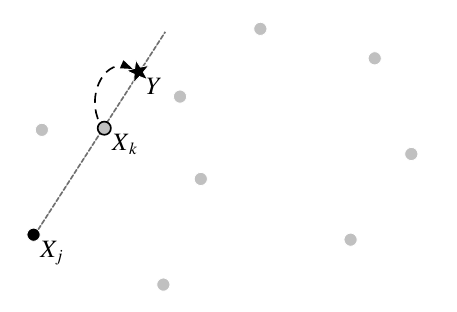
\includegraphics[width=0.8\linewidth]{stretchmove.png}
\caption{Figure 2 from Goodman and Weare (2010).}
\end{figure}
\end{columns}
\end{frame}


%--------------------------------------------

\begin{frame}
\frametitle{Results}
\begin{itemize}
\item Synthetic data
\item Posterior probability distributions
\end{itemize}
\end{frame}


\begin{frame}
\frametitle{Synthetic data}

\begin{itemize}
\item We have generated a synthetic data similar to \source \ using the pulse profile model.
\item Parameters assumed to be physically reasonable
\item The variability amplitude $A$ determined mainly by observer inclination $i$ and spot co-latitude $\thetas$:
\end{itemize}
\be \label{eq:amplitude}
A = \frac{F_{\mathrm{max}} - F_{\mathrm{min}}} {F_{\mathrm{max}} + F_{\mathrm{min}}}
\ee %https://arxiv.org/pdf/astro-ph/0510038v2.pdf
\be \label{eq:amplitude_incthet}
A \approx \frac{(1-\rg/R)\sin i \sin \thetas}{\rg/R+(1-\rg/R)\cos i \cos \thetas}.
\ee 

%\item Assume uniform or non-uniform prior probability distributions for parameters
%\item 
%\item Obtain posterior probability distributions for the parameters using ensemble sampler


%\end{itemize}
\end{frame}


\begin{frame}
\frametitle{Synthetic data}


\be \label{eq:amplitude_incthet}
A \approx \frac{(1-\rg/R)\sin i \sin \thetas}{\rg/R+(1-\rg/R)\cos i \cos \thetas}.
\ee 
\begin{itemize}
\item Switching $i$ and $\thetas$ has no effect on $A$.
\item However, the variability of polarized flux depends on $i$ and $\thetas$ separately.
\item To study this, we have created two datasets which differ only in $i$ and $\thetas$.
\item We assume either uniform or non-uniform prior probability distributions for parameters.
\item We obtain posterior probability distributions for the parameters using the ensemble sampler.


\end{itemize}
%\item Assume uniform or non-uniform prior probability distributions for parameters
%\item 
%\item Obtain posterior probability distributions for the parameters using ensemble sampler


%\end{itemize}
\end{frame}



%-----------------------------------------------------

%-----------------------------------------------------
\begin{frame}

\begin{center}
\frametitle{Synthetic data}
\begin{table}
  \caption{Paramters of the synthetic datasets.}
\label{table:params}
\begin{center}
  \begin{tabular}{| c | c |}
    \hline
     Parameter & Value\\ \hline
      Radius $R$ & 12.0 km  \\ \hline
      Mass $M$ & 1.5 $\msun$  \\ \hline
      Inclination $i$ & 5 $\degree$ or 75 $\degree$ \\ \hline
      Spot colatitude $\thetas$ & 75 $\degree$ or 5 $\degree$ \\ \hline
      Spot angular size $\rho$ & 10.0 $\degree$  \\ \hline
      Distance $D$ & 2.5 kpc \\ \hline
      Temperature $T_{\mathrm{eff}}$ & 2.0 keV \\

    \hline
  \end{tabular}
  \end{center} 

  \end{table}
\end{center}

\end{frame}
%--------------------------------------------

\begin{frame}
\frametitle{Synthetic data}
\begin{columns}[c] % The "c" option specifies centered vertical alignment while the "t" option is used for top vertical alignment
\column{.45\textwidth} 
\begin{figure}
%\includegraphics[width=0.7\linewidth]{neutron-star-magnetic-field.jpg}
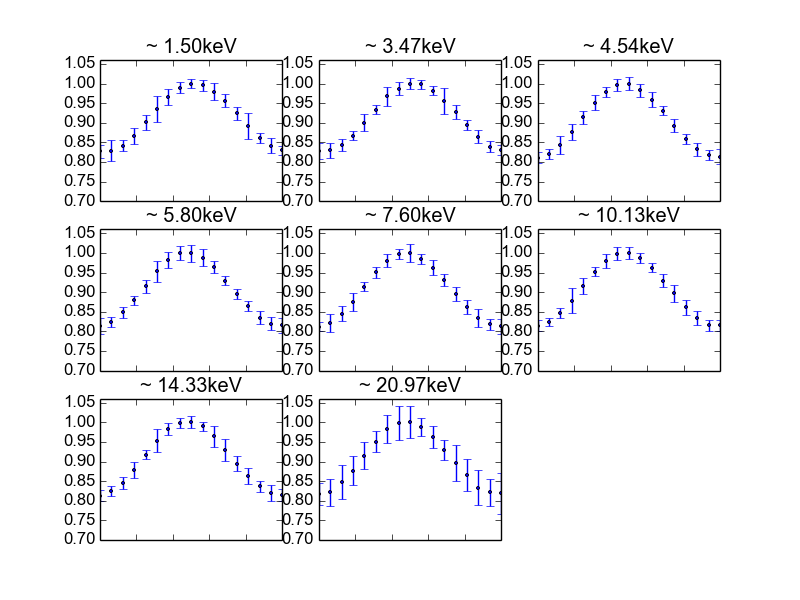
\includegraphics[width=1.2\linewidth]{synt_sax_eq2.png}
\caption{Equatorial spot}
\end{figure}
\column{.45\textwidth} 
\begin{figure}
%\includegraphics[width=0.7\linewidth]{neutron-star-magnetic-field.jpg}
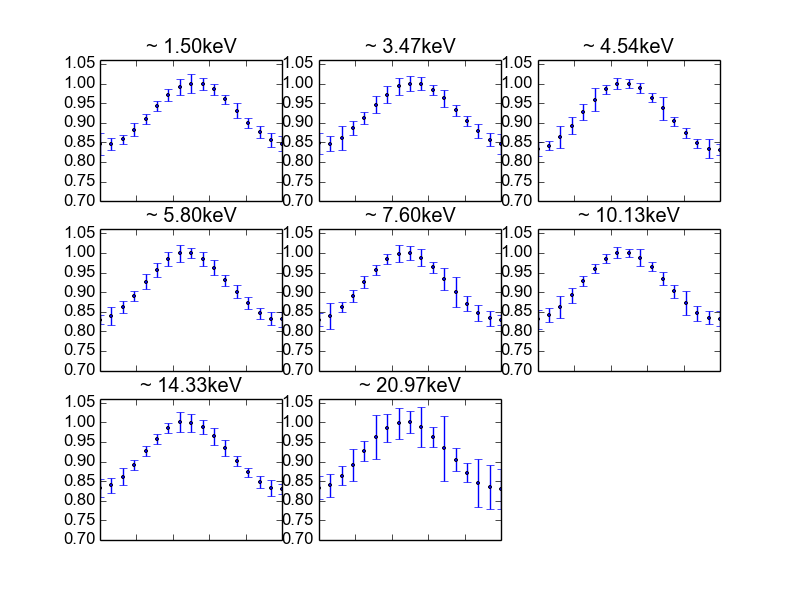
\includegraphics[width=1.2\linewidth]{synt_sax_pol2.png}
\caption{Polar spot}
\end{figure}
\end{columns}

\end{frame}

%-----------------------------------------------------


\iffalse
%--------------------------------------------

\begin{frame}
\frametitle{Burn-in and autocorrelation}
\begin{columns}[c] % The "c" option specifies centered vertical alignment while the "t" option is used for top vertical alignment
\column{.45\textwidth} 
\begin{figure}
%\includegraphics[width=0.7\linewidth]{neutron-star-magnetic-field.jpg}
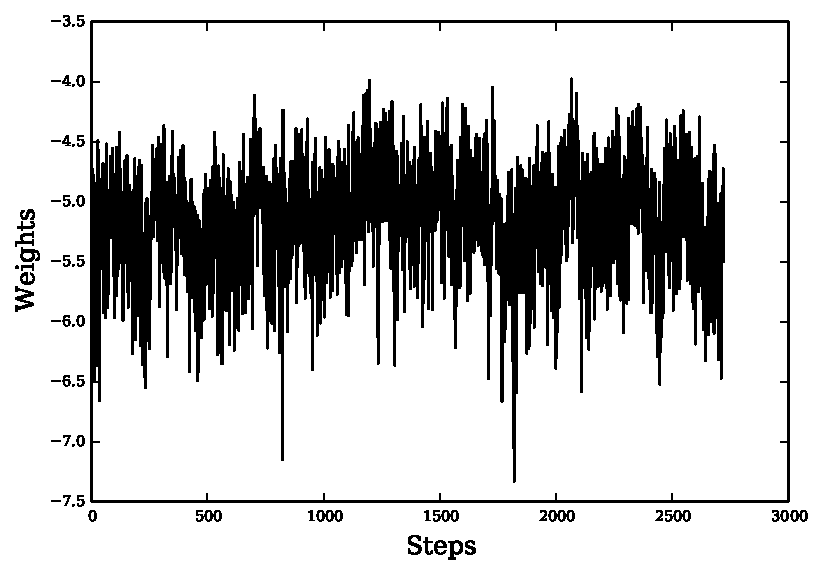
\includegraphics[width=1.1\linewidth]{weights_example.pdf}
\caption{Log-likelihoods after burn-in removal.}
\end{figure}
\column{.45\textwidth} 
\begin{figure}
%\includegraphics[width=0.7\linewidth]{neutron-star-magnetic-field.jpg}
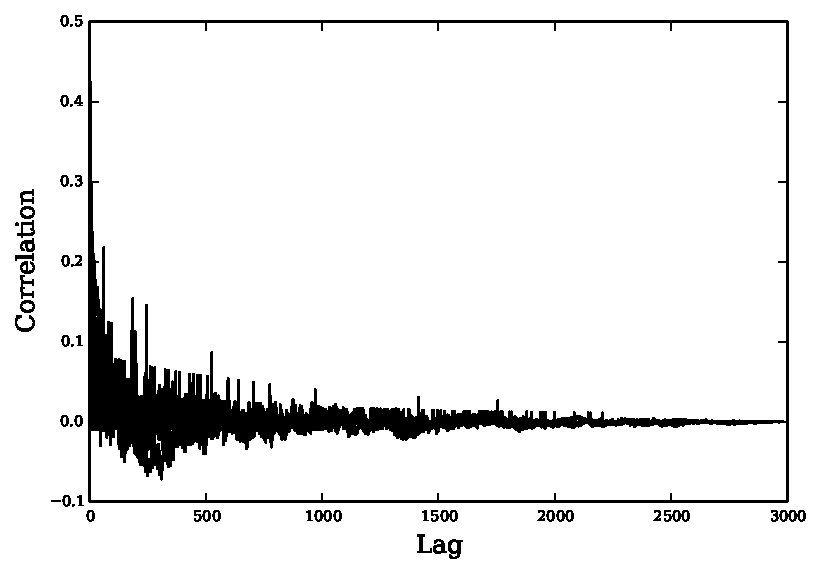
\includegraphics[width=1.1\linewidth]{ac_fpol.pdf}
\caption{Autocorrelation.}
\end{figure}
\end{columns}

\end{frame}

%-----------------------------------------------------

\begin{frame}
\frametitle{Sampling methods}
\begin{itemize}
%\item Marginalization over different phaseshifts
\item Four simulations running parallel on 22 processors
\item In each chain (processor) ~ 70 000 samples out of which 20 000 removed ("burn-in") and thinned with factor 5 (to remove autocorrelation)

\end{itemize}

\end{frame}

\fi
%--------------------------------------------

\begin{frame}
\frametitle{Posterior probability distributions}

\begin{figure}
%\includegraphics[width=0.7\linewidth]{neutron-star-magnetic-field.jpg}
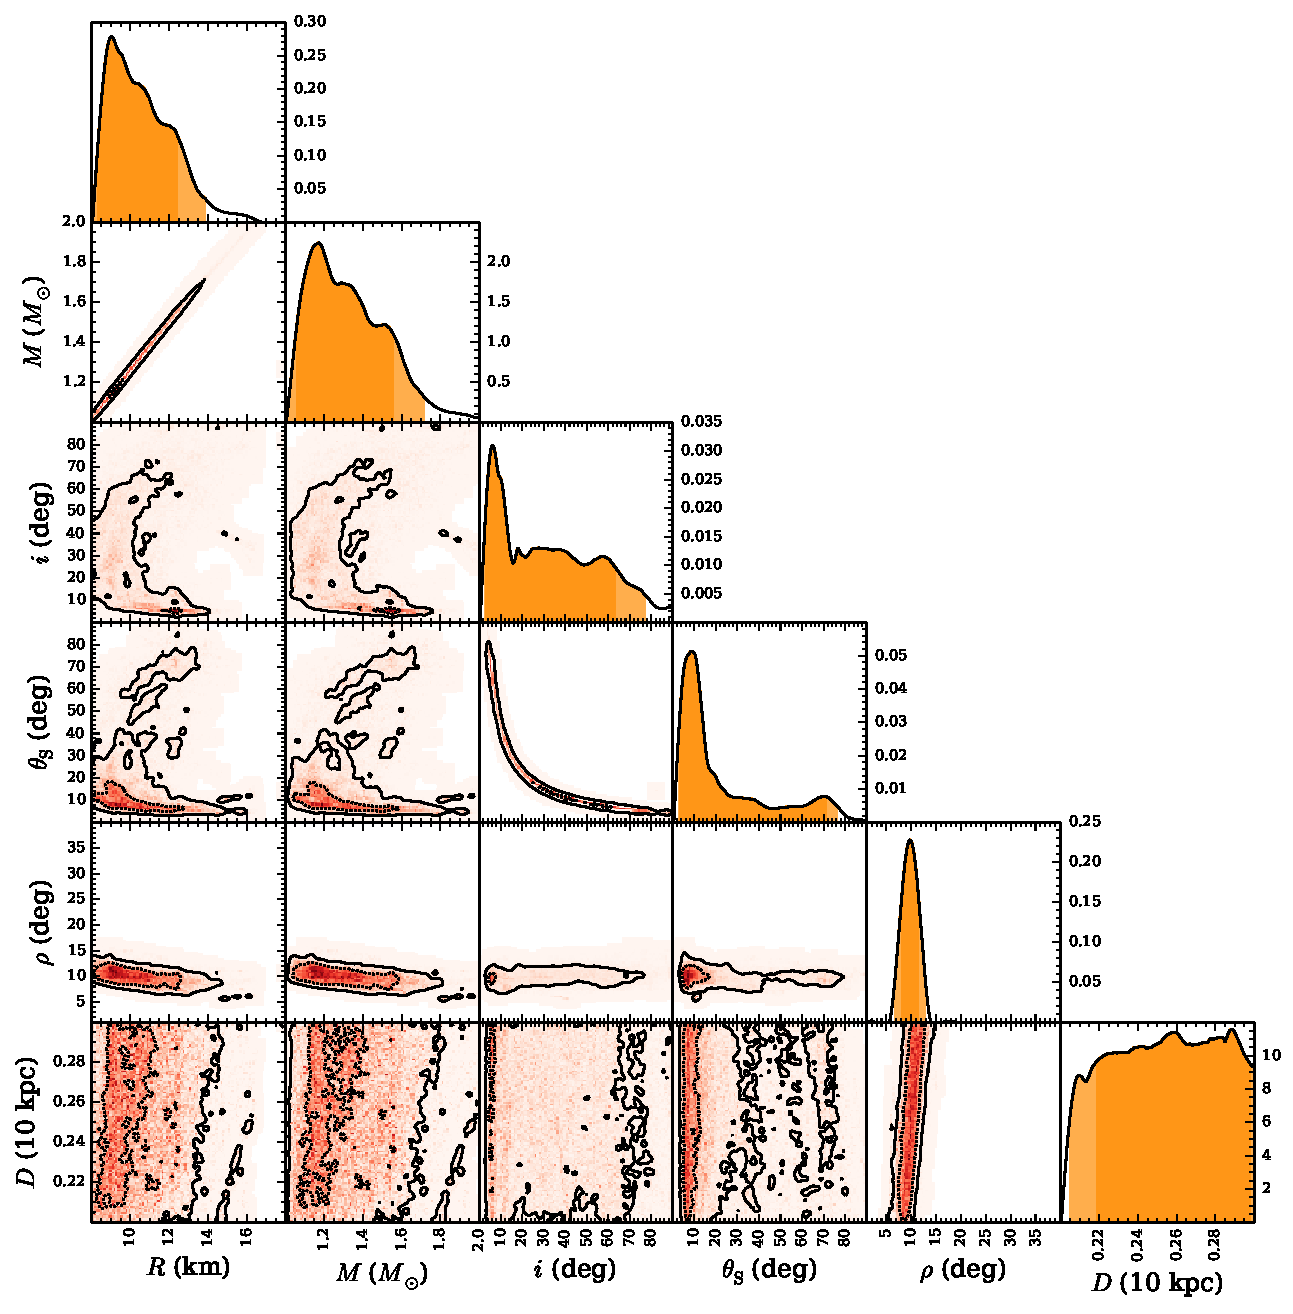
\includegraphics[width=0.55\linewidth]{fpolf.pdf}
\caption{Polar spot with only uniform priors.}
\end{figure}

\end{frame}

%-----------------------------------------------------

%--------------------------------------------

\begin{frame}
\frametitle{Posterior probability distributions}

\begin{figure}
%\includegraphics[width=0.7\linewidth]{neutron-star-magnetic-field.jpg}
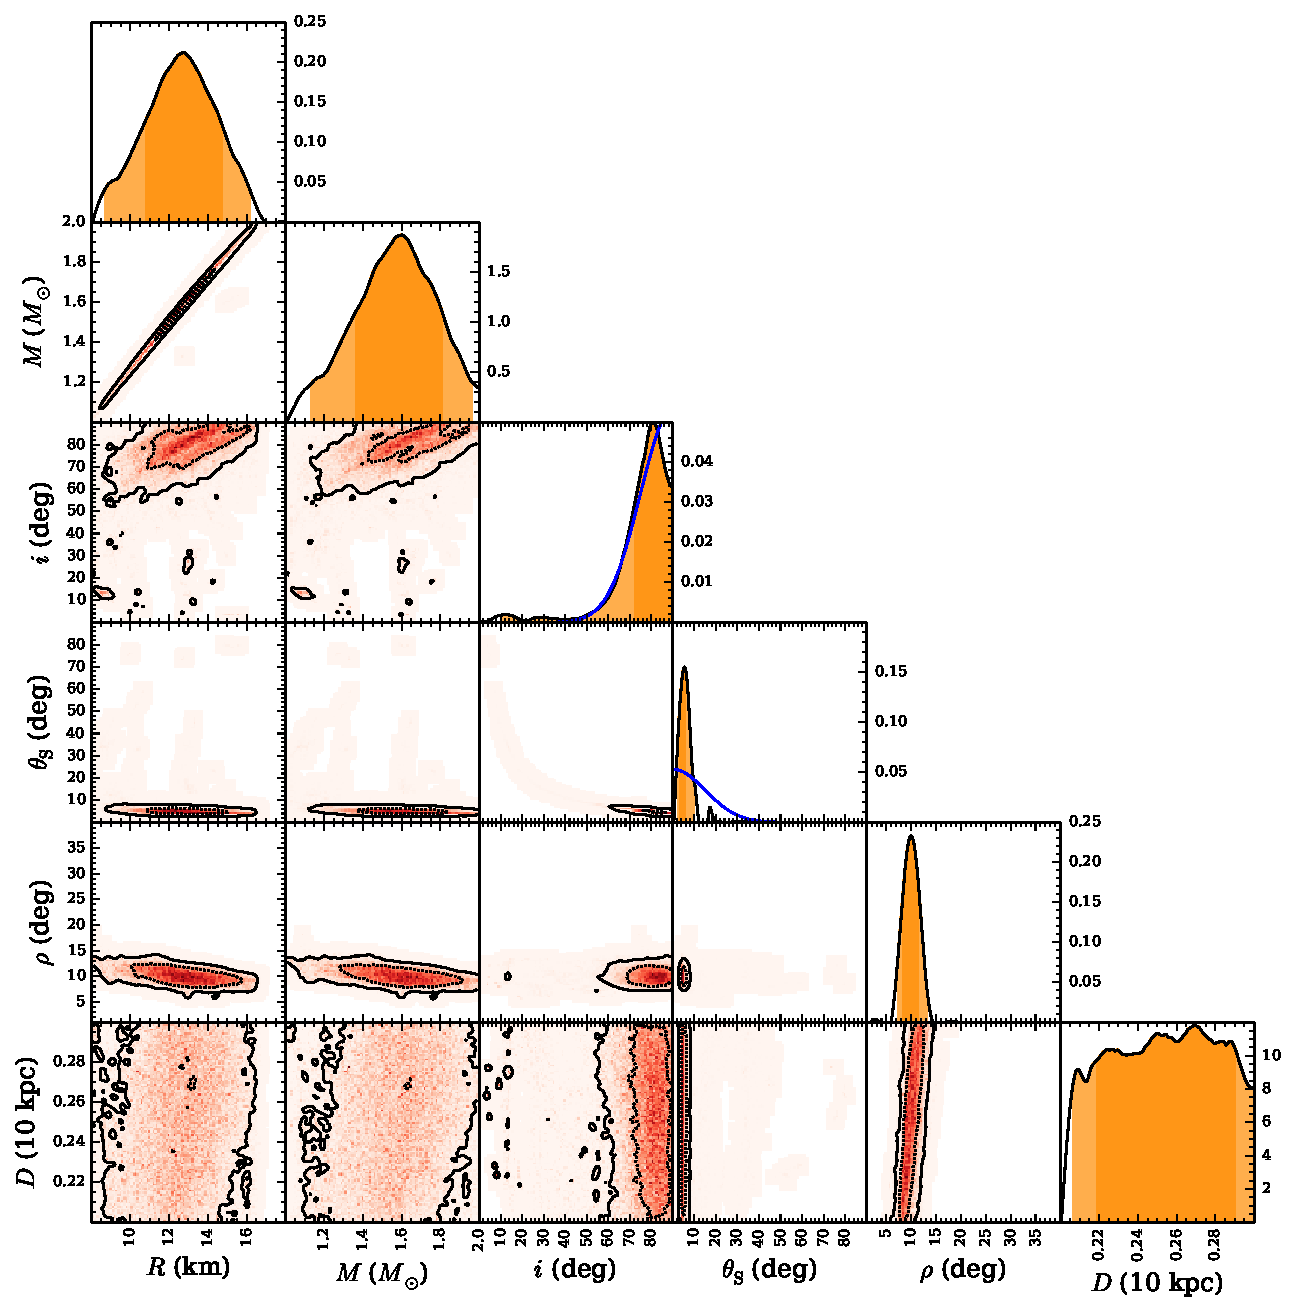
\includegraphics[width=0.55\linewidth]{fpolprf.pdf}
\caption{Polar spot with non-uniform $i$ and $\thetas$ priors (blue lines).}
\end{figure}

\end{frame}

%-----------------------------------------------------

%--------------------------------------------

\begin{frame}
\frametitle{Posterior probability distributions}

\begin{figure}
%\includegraphics[width=0.7\linewidth]{neutron-star-magnetic-field.jpg}
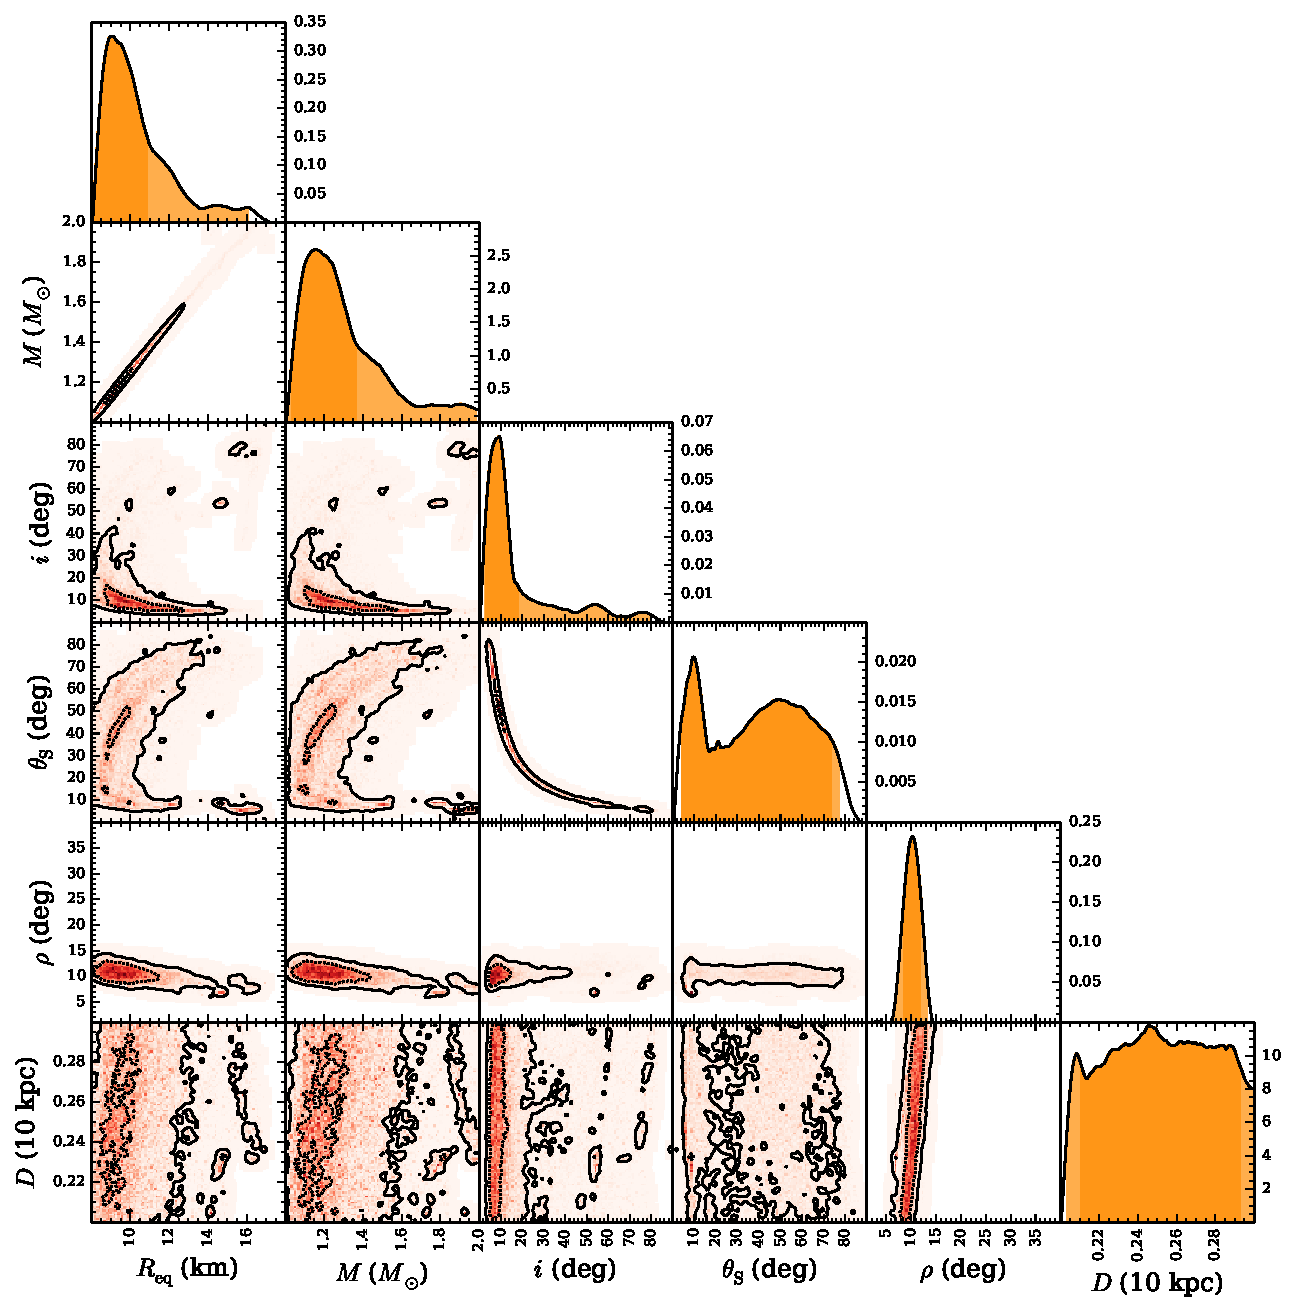
\includegraphics[width=0.55\linewidth]{feqf.pdf}
\caption{Equatorial spot with only uniform priors.}
\end{figure}

\end{frame}

%-----------------------------------------------------


%--------------------------------------------

\begin{frame}
\frametitle{Posterior probability distributions}

\begin{figure}
%\includegraphics[width=0.7\linewidth]{neutron-star-magnetic-field.jpg}
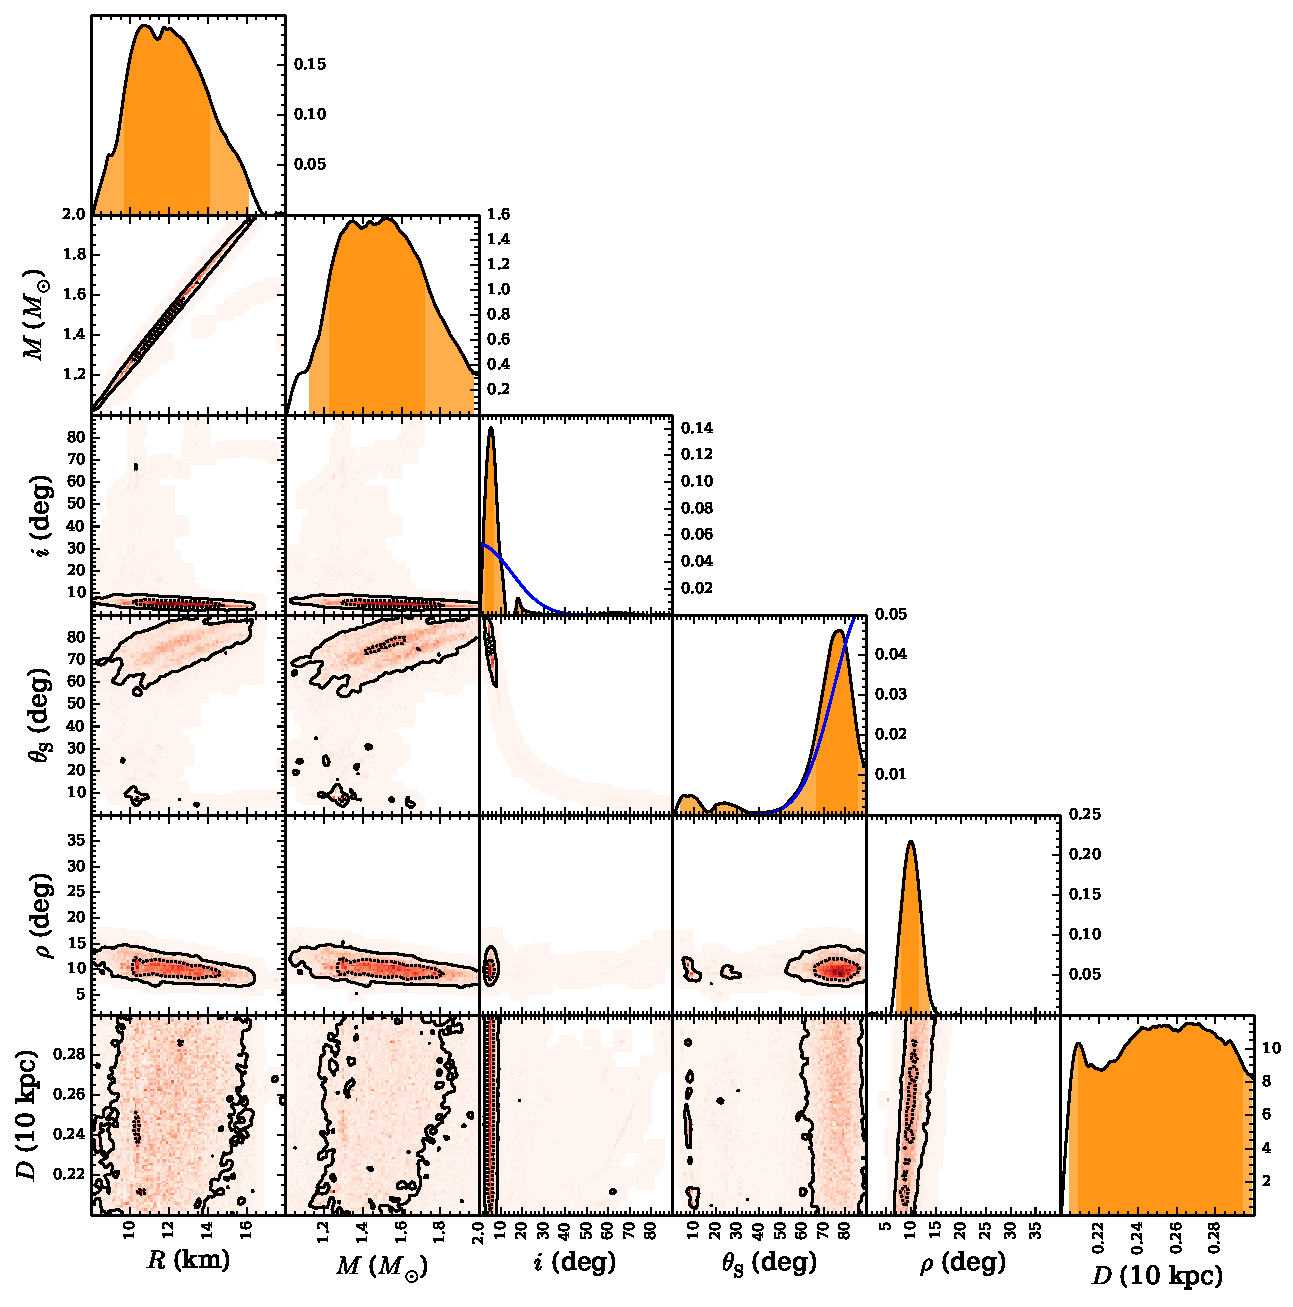
\includegraphics[width=0.55\linewidth]{feqprf.pdf}
\caption{Equatorial spot with non-uniform $i$ and $\thetas$ priors (blue lines).}
\end{figure}

\end{frame}

%-----------------------------------------------------

\begin{frame}
\frametitle{Results}
\begin{itemize}
\item Only upper limits for masses and radii when only non-uniform priors
\item Both upper and lower limits when prior information for $i$ and $\thetas$ applied
\item Correct $i-\thetas$ solution not found without prior information.
\item The size of the spot is well constrained but the distance is not.
\end{itemize}

\end{frame}


\begin{frame}
\frametitle{Summary}
\begin{itemize}
\item AMXPs show coherent oscillations at the spinning frequency of the pulsar.
\item These oscillations may be used to constrain masses and radii of pulsars.
\item Tighter constraints for mass and radius from polarization
\item Future
\begin{itemize}
\item Develope the model
\item From synthetic to real observations
\end{itemize} 

\end{itemize}
\end{frame}













\iffalse

%------------------------------------------------
\section{Second Section}
%------------------------------------------------

\begin{frame}
\frametitle{Table}
\begin{table}
\begin{tabular}{l l l}
\toprule
\textbf{Treatments} & \textbf{Response 1} & \textbf{Response 2}\\
\midrule
Treatment 1 & 0.0003262 & 0.562 \\
Treatment 2 & 0.0015681 & 0.910 \\
Treatment 3 & 0.0009271 & 0.296 \\
\bottomrule
\end{tabular}
\caption{Table caption}
\end{table}
\end{frame}

%------------------------------------------------

\begin{frame}
\frametitle{Theorem}
\begin{theorem}[Mass--energy equivalence]
$E = mc^2$
\end{theorem}
\end{frame}

%------------------------------------------------

\begin{frame}[fragile] % Need to use the fragile option when verbatim is used in the slide
\frametitle{Verbatim}
\begin{example}[Theorem Slide Code]
\begin{verbatim}
\begin{frame}
\frametitle{Theorem}
\begin{theorem}[Mass--energy equivalence]
$E = mc^2$
\end{theorem}
\end{frame}\end{verbatim}
\end{example}
\end{frame}

%------------------------------------------------

\begin{frame}
\frametitle{Figure}
Uncomment the code on this slide to include your own image from the same directory as the template .TeX file.
\begin{figure}
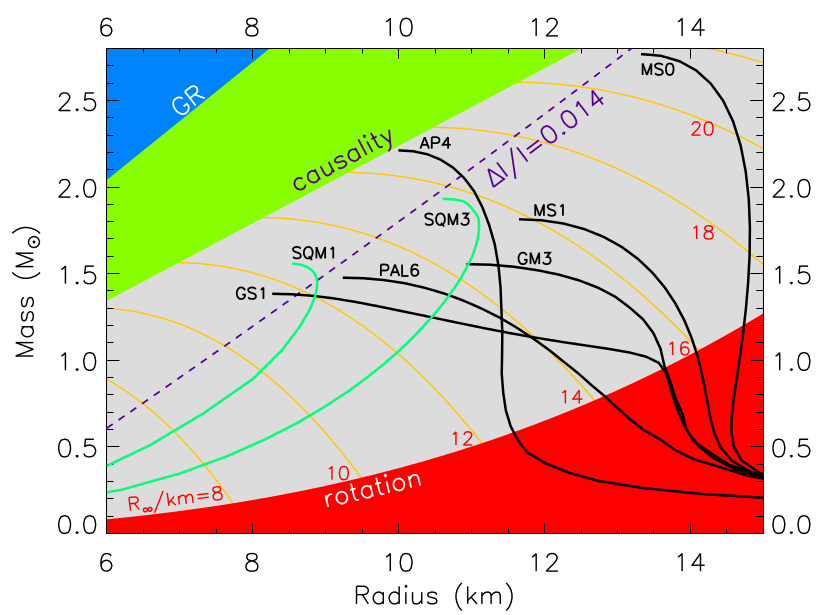
\includegraphics[width=0.8\linewidth]{eos_mr.png}
\end{figure}
\end{frame}

%------------------------------------------------

\fi
%\begin{frame}[fragile] % Need to use the fragile option when verbatim is used in the slide
%\frametitle{Citation}
%An example of the \verb|\cite| command to cite within the presentation:\\~

%This statement requires citation \cite{p1}.
%\end{frame}

%------------------------------------------------

%\begin{frame}
%\frametitle{References}
%\footnotesize{
%\begin{thebibliography}{99} % Beamer does not support BibTeX so references must be inserted manually as below
%\bibitem[Smith, 2012]{p1} John Smith (2012)
%\newblock Title of the publication
%\newblock \emph{Journal Name} 12(3), 45 -- 678.
%\end{thebibliography}
%}
%\end{frame}

%------------------------------------------------

\begin{frame}
\Huge{\centerline{The End}}
\end{frame}

%----------------------------------------------------------------------------------------

\end{document}